\chapter{System Integration}

This section of the report outlines the plan for integrating both the physical hardware components and the software architecture of the greenhouse system. It begins with the wiring layout of all electronic components, followed by a description of the software framework and control logic that will govern the system operation. This section on system integration demonstrates how the various subsystems, sensors, actuators, and controllers, work together to achieve the overall functionality of the greenhouse. It also provides a clear roadmap for implementation, troubleshooting, and future scalability.

\section{Wiring}

The battery provides a 12V power rail to any components that require it. This 12V supply is connected to the Common (COM) terminals of the relay module. When activated by the microcontroller, each relay allows current to flow from the COM terminal to the Normally Open (NO) terminal, supplying 12V to the connected device. On the input side of the relay module, the VDD pin must be connected to a 5V power source, and the GND pin to ground. The four input pins labeled IN1–IN4 are connected to general-purpose I/O (GPIO) pins on the microcontroller, specifically GPIO 38,37,47 and 48, allowing the relays to be toggled via 3.3V logic signals.

These relays control the 12V-powered components: airflow fans, heater fan, grow light, and solenoid valve. Each of these devices requires a connection to ground on their negative terminal, which is wired to the negative terminal of the battery. A common ground rail ensures all components share the same electrical ground reference. The wiring schematic can be seen in the figure below


\begin{landscape}
	\begin{figure}[p]
		\centering
		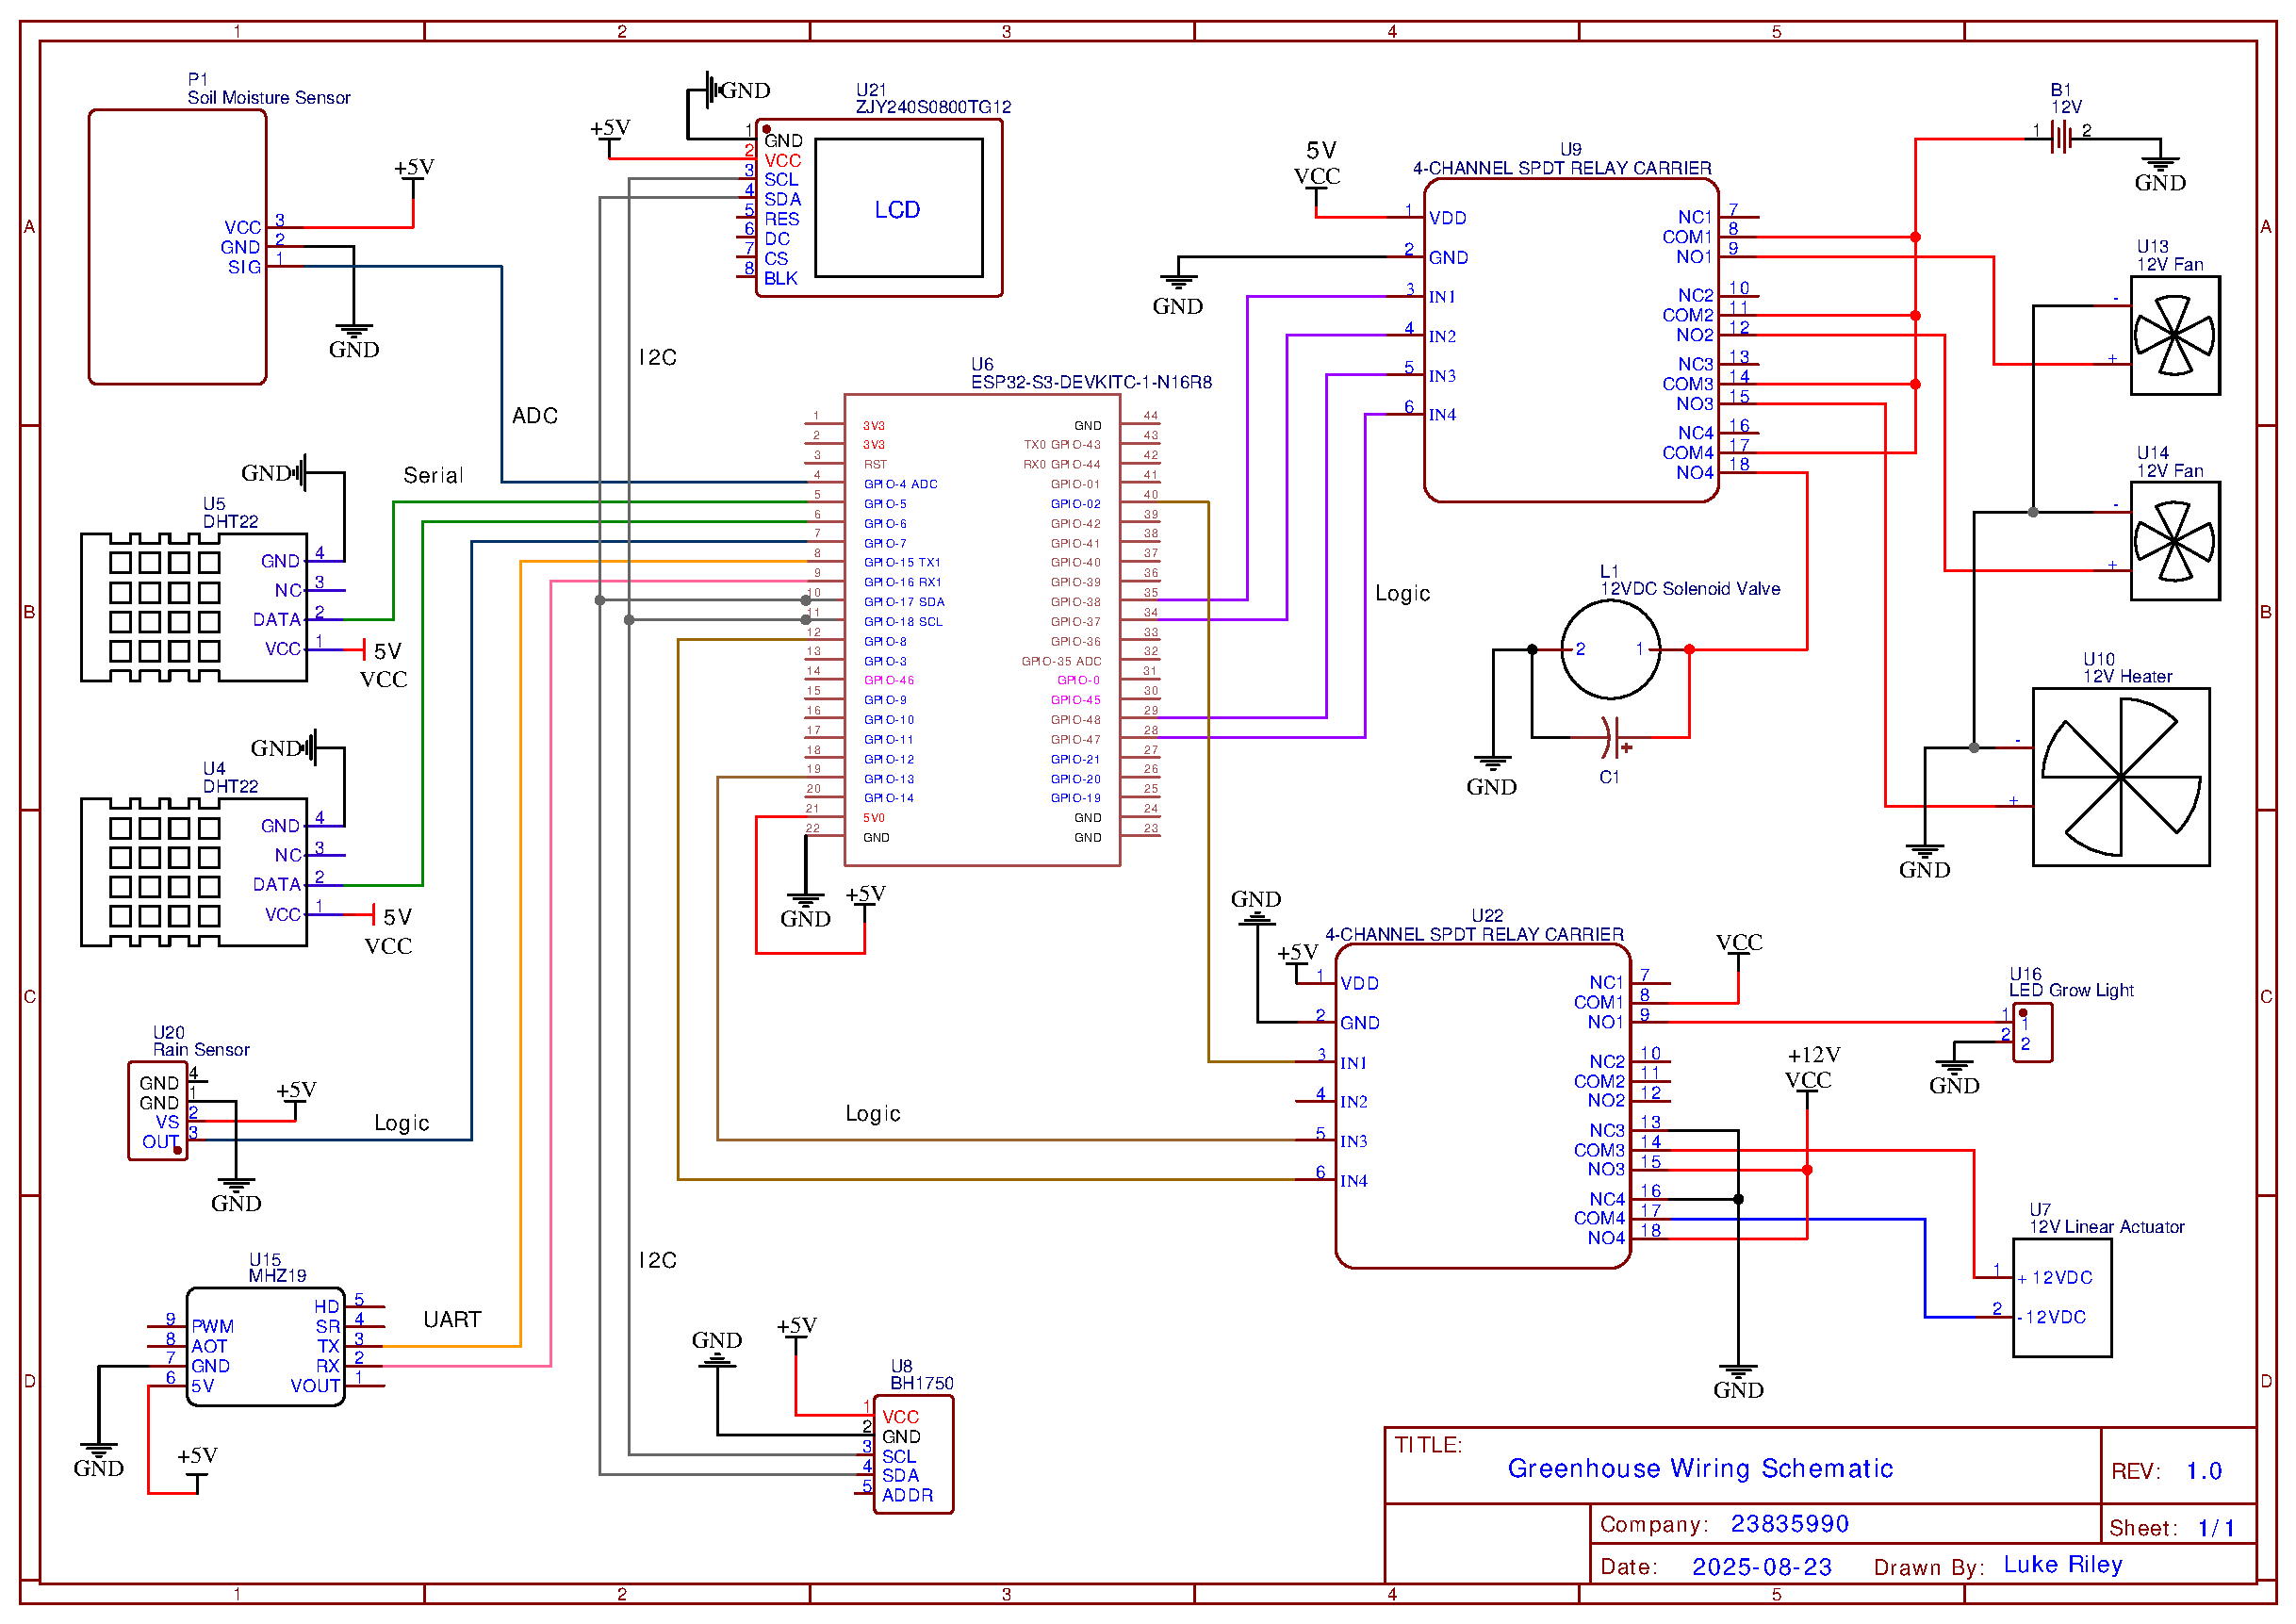
\includegraphics[width=\linewidth]{figs/wiringpd.pdf}
		\caption{Wiring schematic}
		\label{fig:lcd_screen}
	\end{figure}
\end{landscape}

For the linear actuator, bidirectional motion is achieved by reversing the polarity of the supply voltage using two channels of the relay module. GPIO 8 and GPIO 13 of the microcontroller are connected to input pins IN3 and IN4 of the relay module, respectively. The 12V supply is wired to the Normally Open (NO) terminals of both relays, while the actuator leads are connected to the Common (COM) ports. The Ground connection is tied to the Normally Closed (NC) terminals of each relay. With this configuration, switching the relays in different states alternates the polarity applied to the actuator, enabling both extension and retraction.

Other components and sensors require a 5V supply. A buck regulator is used to step down the 12V input efficiently, avoiding the high energy loss associated with voltage dividers. The regulator’s VIN is connected to the 12V rail, and its GND pins are tied to ground. The VOUT pin is connected to a 5V power rail that supplies all 5V-dependent components. Before connecting any loads, the regulator should be calibrated by measuring the output with a multimeter and adjusting the onboard potentiometer until the desired 5V output is reached.

The DHT22 sensors each require a 5V VCC connection, ground to GND, and a data line connected to GPIO 5 and 6 respectively, using digital communication. The soil moisture sensor is similarly powered with 5V to VCC, ground to GND, and its data line connected to GPIO 4. The BH1715 light sensor communicates via the I\textsuperscript{2}C protocol and is connected to 5V and ground, with SDA and SCL lines wired to GPIO 17 and 18 respectively. The rain sensor outputs a logical high coltage level of 3,3V when water is deticted, accordingly GPIO 7 is set as an input pin to read the logic level. The CO\textsubscript{2} sensor requires a 5V supply to its 5V pin, GND to ground, and TX/RX lines connected to UART-compatible GPIO pins—GPIO 15 and 16 in this case.

For local display of environmental readings, an I²C LCD module is used. The module requires 5V on its VCC pin and ground on GND. Communication with the microcontroller is achieved via the I²C protocol, with GPIO 17 connected to the SDA line and GPIO 18 to the SCL line. This configuration reduces the number of required connections compared to a parallel LCD, while still enabling reliable display of real-time sensor data. A wiring schematic is provided below.

\section{Software Framework and Control Logic}

This section outlines the software design framework for the greenhouse system. The accompanying flowcharts illustrate the sequence of tasks and decision-making processes implemented on the microcontroller. These flowcharts serve to simplify the development of complex control algorithms—particularly those involving multiple variables with competing operational requirements.

In certain situations, control actions are prioritized based on environmental conditions. For example, if the internal temperature exceeds the setpoint while soil moisture levels remain adequate, the misting system may still be activated to assist with cooling. In such cases, temperature regulation is prioritized over soil moisture conservation.

The control logic is structured into distinct modules, arranged in approximate order of priority: \textit{Principal Control}, \textit{Temperature Control}, \textit{Airflow Control}, \textit{Humidity Control}, \textit{Lighting Control}, and \textit{Air Quality Control}.

\begin{figure}[H]
\centering
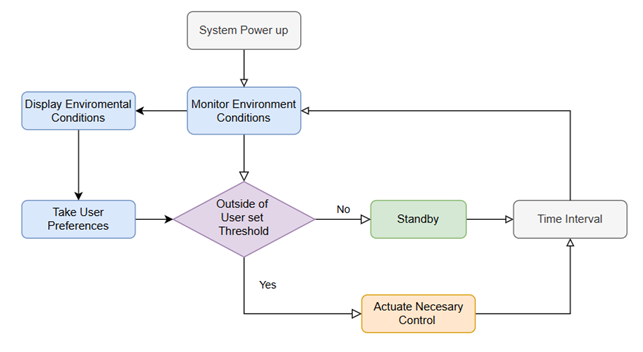
\includegraphics[width=0.85\textwidth]{figs/soft1.png} % Update path/filename as needed
\caption{Principal Control Flowchart}
\label{fig:principle_control_flowchart}
\end{figure}

Principal Control involves monitoring internal and external environmental conditions, to inform decisions about which components need to be actuated in response to undesirable conditions. These environmental readings are displayed to the user, who can then set custom threshold values based on the specific requirements of the plants being cultivated. When any measured condition falls outside the user-defined thresholds, the system responds by activating the appropriate control mechanisms. If no user preferences are provided, the system defaults to a broad, general-purpose set of control setpoints suitable for common plant types.

\begin{figure}[htbp]
    \centering
    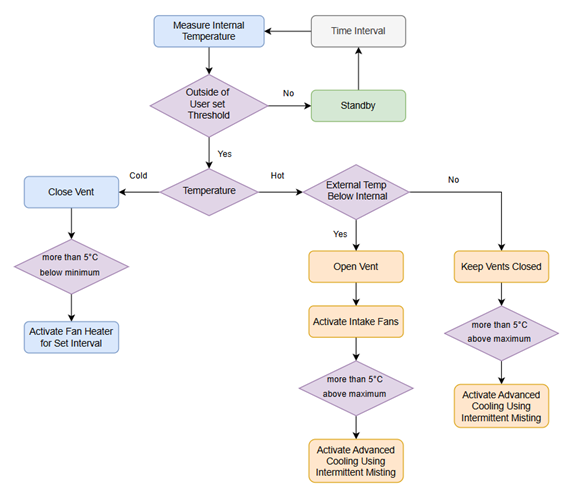
\includegraphics[width=0.8\textwidth]{figs/soft2.png}
    \caption{Temperature control}
    \label{fig:temperature_control}
\end{figure}

\begin{figure}[htbp]
    \centering
    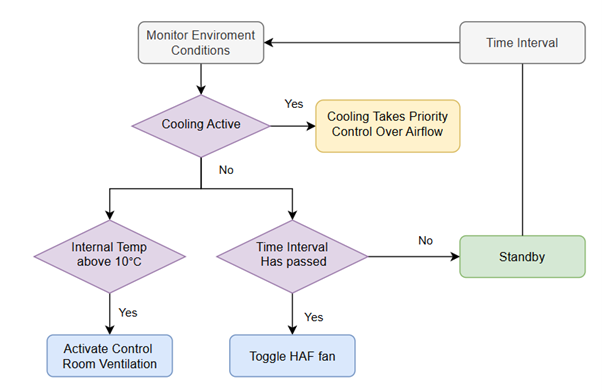
\includegraphics[width=0.7\textwidth]{figs/soft3.png}
    \caption{Airflow control}
    \label{fig:airflow_control}
\end{figure}

\begin{figure}[htbp]
    \centering
    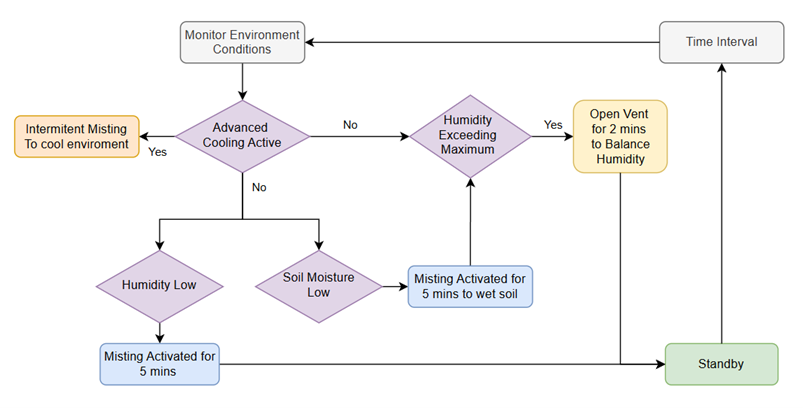
\includegraphics[width=0.8\textwidth]{figs/soft4.png}
    \caption{Irrigation control}
    \label{fig:irrigation_control}
\end{figure}

\begin{figure}[htbp]
    \centering
    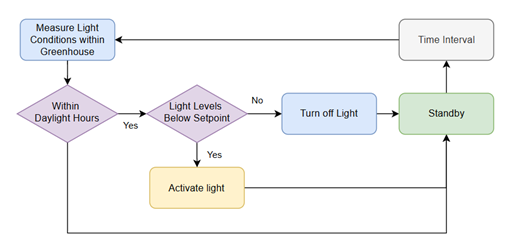
\includegraphics[width=0.7\textwidth]{figs/soft5.png}
    \caption{Light control}
    \label{fig:light_control}
\end{figure}

\begin{figure}[htbp]
    \centering
    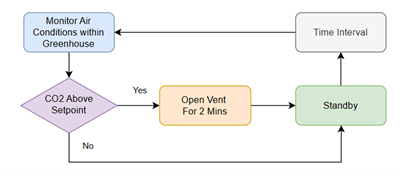
\includegraphics[width=0.6\textwidth]{figs/soft6.png}
    \caption{Air quality Control}
    \label{fig:air_quality_control}
\end{figure}

The inclusion of these flowchart diagrams streamlines the programming of the microcontroller's control logic by providing a clear framework for implementation, reducing the likelihood of debugging issues caused by conflicting decision-making processes.